\section{Einleitung}
Der Einsatz von Robotern prägt zunehmend den Arbeitsmarkt und beeinflusst die Art und Weise wie Unternehemn ihre Prozesse gestalten. Diese Entwicklung beschränkt sich nicht nur auf die Industrie und den Verbrauchermarkt, sondern immer zunehmender auch auf die Dienstleistungsbranche. So ist der Absatz an Service Robotern für professionelle Anwendungen 2022 laut der International Federation of Robotics \cite{IFR2023} um 48\% gestiegen. Hierbei gibt es laut der \ac{IFR} eine Abgrenzung zu Service Robotern für Verbraucher, bei denen der Absatz 2022 gesunken ist \cite[S.~37]{WorldRobotics2023} und Industrie Robotern bei denen der Absatz 2022 gestiegen ist \cite[S.~9]{WorldRobotics2023}. Aufgrund der Stichprobenentnahme für die Berechnung des Absatzes ist keine genauere Vergleichbarkeit zwischen den Absatzdaten möglich. Das Wachstum des Absatzes wird laut der \ac{IFR} \cite[S.~36]{WorldRobotics2023} unter anderem durch eine gesteigerte Nachfrage getrieben, die auf einen Mangel an Arbeitskräften zurückzuführen ist. Laut der \ac{BA} \cite{BA2024} ist beispielsweise die Menge unbesetzter Arbeitsplätze in Deutschland in den letzten 12 Jahren um ca. zwei Drittel gestiegen und trotz des Rückgangs um ~9\% im Jahr 2023 weiter auf einem hohen Stand. Service Roboter bieten die Möglichkeit diesen Mangel an Arbeitskräften zu mitigieren, da sie eine effiziente Unterstützung der Arbeiter bieten und so die Produktivität erhöhen. Hierbei ersetzen Service Roboter die Menschen meistens nicht vollständig, sondern unterstützen diese nur. Laut Sprenger \cite[S.~272]{Sprenger2015} muss ein Transportroboter beispielsweise von einem Menschen mitgeteilt bekommen was von wo nach wo transportiert werden soll, kann den Transport dafür dann aber vollständig automatisch durchführen. Auf diese Weise haben die Menschen mehr Zeit für andere Aufgaben wie die Kundenbetreuung

\subsection{Hintergrund und Motivation}
Insbesondere in der Gastronomie gibt es einen großen Personalmangel. Dieser ist zum Teil auf die Corona-Pandemie zurückzuführen, da in dieser Zeit viele Angestellte in andere Berufsfelder gewechselt sind. Laut dem Institut der deutschen Wirtschaft \cite{BA2024} - welches sich auf Daten der \ac{BA} bezieht - sind während des Pandemiejahrs 2020 216.000 Arbeiter aus dem Gastgewerbe in ein anderes Berufsfeld gewechselt. Das Gastgewerbe schließt hierbei neben der Gastronomie auch die Hotellerie und Tourismus mit ein. Der Personalmangel macht den Einsatz von Service Robotern in der Gastronomie besonders attraktiv. Diese können dort besonders gut Kellneraufgaben übernehmen und so das Personal entlasten. Das steigert nicht nur die Produktivität, sondern verbessert zusätzlich auch die Arbeitsbedingungen. Wie bereits erwähnt agieren die Transportroboter hierbei nicht vollständig autonom, sondern müssen ihre Aufträge von Menschen mitgeteilt bekommen. Man braucht aber nicht nur die Möglichkeit Robotern Aufgaben mitzuteilen, sondern auch die Möglichkeit Roboter zu Orten und herauszufinden was die Roboter aktuell machen.
% TODO Formulierung verbessern; insgesamt Struktur verbessern, da auch Teile aus vorherigem Abschnitt wiederholt werden.

In dieser Arbeit wird sich speziell mit den Lieferrobotern von Pudu beschäftigt, da diese dem Author zur verfügung stehen. Pudu bietet verschiedene Lieferroboter, an die in der Gastronomie zur Entlastung der Kellner eingesetzt werden können \cite{PUDU2024}. Für diese Arbeit wird auf eine bereits entwickelte API - das \ac{BCB} - zurückgegriffen, die Endpunkte bereitstellt, mit denen unteranderem Lieferaufträge gegeben und Daten der Roboter abgerufen werden können.

% Im Zuge der weiteren Vertiefung dieses Themas wird im Verlauf der Arbeit genauer auf die Rolle von Service Robotern als Antwort auf den Fachkräftemangel eingegangen. Hierbei werden nicht nur die Vorteile, sondern auch die Herausforderungen und mögliche Lösungsansätze beleuchtet, um eine umfassende Perspektive auf die Thematik zu gewährleisten.

\subsection{Zielsetzung und Forschungsfrage}
Diese Arbeit setzt an dem Punkt an und verfolgt entsprechend das Ziel eine Anwendung zu konzeptionieren und prototypisch zu implementieren, die die Möglichkeit bietet Service Roboter zu steuern und verwalten. Diese Anwendung soll eine intuitive Steuerung und Übersicht bieten. Bei der Anwendung soll es sich aufgrund verschiedener Vorteile gegenüber nativen Apps um eine Webanwendung handeln. So können Webanwendungen plattformunabhängig genutzt werden und sind sofort ohne Download und Installation verfügbar. Da diese Anwendung in beliebigen Betrieben einsetzbar sein soll, braucht es auch die Möglichkeit eine Visualisierung des entsprechenden Gebäudes zu erstellen. Für eine bessere übersichtlichkeit soll diese visualisierung 3-dimensinal sein. Das Erstellen eines 3D Modells erfordert klassischerweise technisches Know-How in Modellierungssoftware wie beispielsweise Blender. Dieses fehlt in den meisten Gastronomiebetrieben, weshalb hierfür eine einfacherere Lösung gefunden werden soll. Das Generieren einer 3-dimensionalen Gebäudeübersicht ist entsprechend ein zusätzlicher Schwerpunkt dieser Arbeit.

% TODO Erläutern warum Effizienz/Performance und Benutzerfreundlichkeit nötig sind

Aus der genannten Zielsetzung ergibt sich die folgende Forschungsfrage: Wie kann eine effiziente und benutzerfreundliche Steuerung und Verwaltung von Servicerobotern implementiert werden? Ein besonderer Schwerpunkt liegt hierbei auf der Ausarbeitung einer Methode zur einfachen Generierung von 3D-Modellen, um die Grundlage für die nutzerfreundliche Visualisierung und Navigation in der Webanwendung zu schaffen. Die ausgearbeitete Methode muss nicht zwingend in die Webanwendung integriert werden, sondern kann lediglich ein 3D-Modell generieren, welches dann in der Webanwendung importiert werden kann.


\subsection{Methodik}
Diese Arbeit orientiert sich an dem \ac{DSR} Ansatz nach Hevner. Dieser bietet speziell einen Rahmen für \ac{DSR} im Bereich der Informationssysteme und ist somit für diese Arbeit geeignet. Grundsätzlich ist \ac{DSR} ein iterativer Forschungsansatz, mit dem Lösungen für praktische Probleme, mithilfe der Entwicklung von Artefakten gefunden werden. In dem Fall dieser Arbeit ist das Artefakt der zu entwickelnde Prototyp. 

\subsubsection{Design Science Research nach Hevner}
Bei diesem Unterkapitel handelt es sich um eine Zusammenfassung des \ac{DSR} Ansatz nach Hevner \cite[S.~79-81]{Hevner2004}. Hevners Ansatz besteht aus verschiednene Zyklen:

\begin{itemize}
    \item Relevancy Cycle
    \item Rigor Cycle 
    \item Design Cycle
\end{itemize}

Mit diesen Zyklen wird eine systematische Entwicklung und Bewertung der Artefakte erreicht. Hevners Ansatz berücksichtigt die Umgebung, in der und für die das Artefakt entwickelt wird und die Wissensgrundlage, auf der das Artefakt aufbaut. Diese Wissensgrundlage wird durch die Entwicklung des Artefakts erweitert. Im Folgenden werden die Zyklen, Umgebung und Wissensgrundlage genauer erklärt.

\begin{itemize}
    \item Die Umgebung besteht aus den relevanten Menschen, Organisationen und Technologien. Sie definiert den Problemraum in dem geforscht wird. Aus der Umgebung ergeben sich die organisatorischen Bedürfnisse beziehnungsweise das Problem, dass gelöst werden soll und die Anforderungen an die Lösung.
    \item Die Wissensgrundlage bietet verbildlicht die Rohmaterialien mit denen der Design Cycle durchgeführt werden kann. Im Fall dieser Arbeit bezieht sich das beispielsweise auf mögliche Frameworks mit denen 3D-Modelle in der Webanwendung eingebunden werden können, aber auch auf Methoden für die Auswertung des Prototyps.
    \item Im Design Cycle, wird das Artefakt iterativ entwickelt und ausgewertet. Mithilfe des Relevancy Cylce wird sichergestellt, dass das Artefakt das ursprüngliche Problem löst. Der Rigor Cycle bietet eine Wissensgrundlage auf der aufbauend entwickelt werden kann.
    \item Im Relevancy Cycle wird das Problem beziehungsweise die Anforderungen die sich aus dem Problem ergeben an den Design Cycle übergeben. Das Artefakt, das im Design Cycle entsteht, wird dann in der Umgebung getestet. Hierdurch wird sichergestellt, dass das Artefakt das entsprechende Problem in der Umgebung auch wirklich löst.
    \item Im Rigor Cycle wird die Wissensgrundlage an den Design Cycle übergeben. Mit der Entwicklung des Artefakts entsteht neues Wissen. Dieses erweitert die Wissensbasis. Der zweite Teil des Rigor Cycle ist somit nur für die zukünftige Anwendung relevant.
\end{itemize}

\begin{figure}[H]
    \caption{Design Science Research nach Hevner}\label{fig:DesignScienceResearch}
    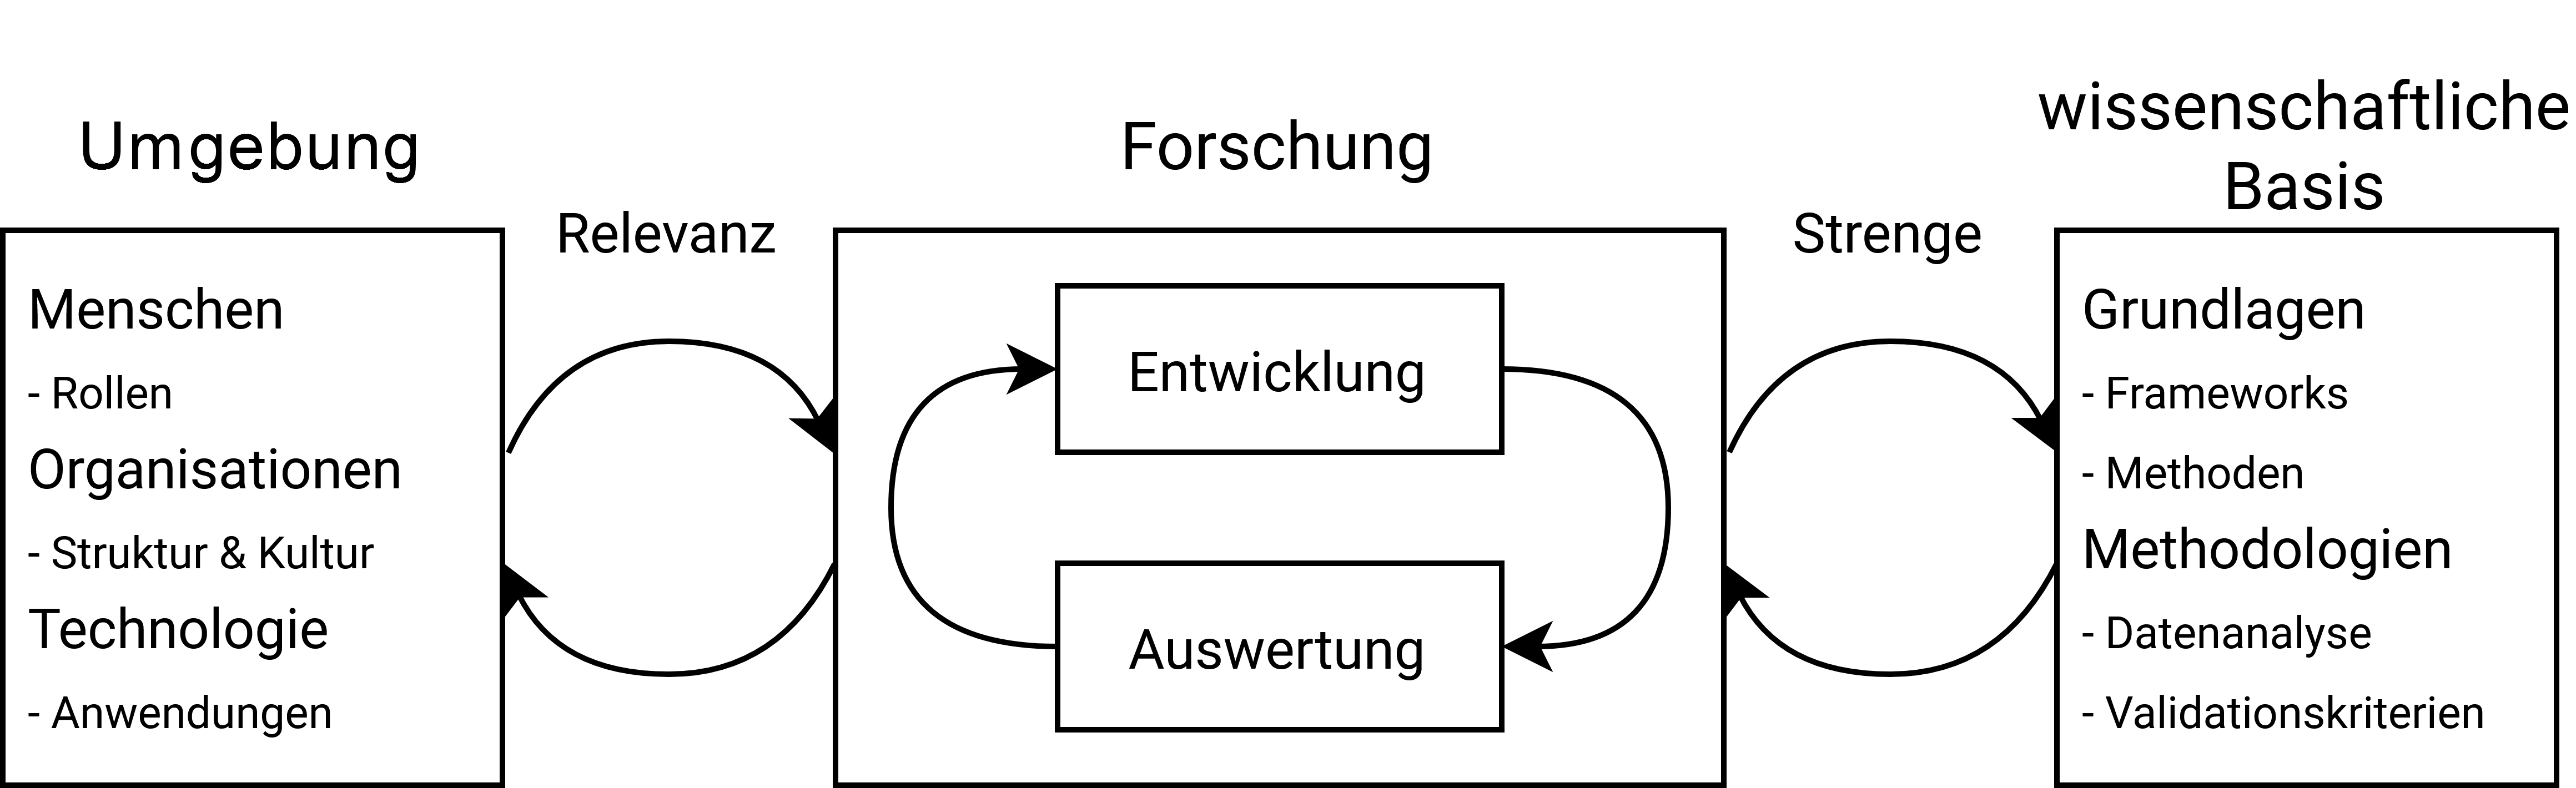
\includegraphics[width=0.9\textwidth]{Design Science Research.png}
    \\
    % TODO Check if "et al." is right
    Quelle: In Anlehnung an Hevner et al. \cite[S.~80]{Hevner2004}
\end{figure}

\subsubsection{Design Science Research im Rahmen der Arbeit}

Die verschiedenen Schritte des \ac{DSR} Ansatz nach Hevner werden in dieser Arbeit mithilfe verschiedener Methoden abgebildet.

\paragraph{Literaturrecherche}
Im ersten Schritt wird eine systematische Literaturrecherche durchgeführt. Mit dieser soll das grundlegende Verständnis über die Umgebung geschaffen werden. So soll insbesondere Wissen zu den Service Robotern gesammelt werden, die in der Gastronomie eingesetzt werden können. Mithilfe der Literaturrecherche soll außerdem die Wissensbasis geschaffen werden. Insbesondere soll Wissen gesammelt werden, mit dem sich eine Lösung für die Generierung von 3D-Modellen von Gebäuden finden lässt. Außerdem soll Wissen zur Einbindung von 3D-Modellen im Web gesammelt werden. Während der Implementierung des Prototyps werden außerdem wahrscheinlich weitere größere technische Probleme auffallen, für die dann entsprechend Wissen gesammelt werden muss. Entsprechend beschränkt sich der Schritt der Literaturrecherche nicht auf den Beginn der Arbeit. Stattdessen wird sie mit dem Auftreten neuer technischer Probleme wiederholt relevant sein.

\paragraph{Anforderungsanalyse}
Daraufhin wird auf Basis des Wissens zur Umgebung im Kontext der Forschungsfrage eine Anforderungsanalyse für den Prototyp erstellt. Durch die Forschungsfrage und den festgelegten Schwerpunkt (3D-Modelle von Gebäuden) stehen bereits verschiedene funktionale und nicht-funktionale Anforderungen fest. So existieren bereits folgende funktionale Anforderungen:

\begin{itemize}
    \item Es soll eine Webanwendung implementiert werden.
    \item Die Anwendung soll eine 3-dimensionale Visualisierung der entsprechenden Gebäude bieten.
\end{itemize}

\begin{samepage}
Außerdem existieren bereits folgende nicht-funktionale Anforderungen:

\nopagebreak
\begin{itemize}
    \item Die Anwendung soll benutzerfreundlich sein.
    \item Die Anwendung soll effizient sein.
\end{itemize}
\end{samepage}

Hierbei muss allerdings basierend auf dem Wissen zur Umgebung noch genauer definiert werden, was unter den beiden Begriffen genau zu verstehen ist. So sollte  präzisiert werden welche Aspekte der Benutzerfreundlichkeit wichtig sind und welche Art von Effizienz gemeint ist.

\paragraph{Umsetzung}
Basierend auf den gesammelten Anforderungen ergeben sich größere technische Herausforderungen. Wie bereits erwähnt sind verschiedene technische Herausforderungen bereits abzusehen, die mithilfe der Wissensbasis gelöst werden sollen. Während der Implementierung des Prototyps können, wie bereits beschrieben weitere Herausforderungen auftreten die mithilfe der sich kontiluierlich entwickelnden Wissensbasis gelöst weren können.

Sobald die Anforderungen definiert sind und die ersten technischen Herausforderungen gelöst sind kann mit der Implementierung des Prototyps begonnen werden. Dieser soll im Verfahren des Rapid Prototypings entwickelt werden, bei denen sich die Implementierung und Evaluierung iterierend abwechseln. Die Benutzerfreundlichkeit und Effizienz des Prototyps soll hierbei durch Usability Tests und Performance Tests evaluiert werden.
